\chapter{Thực nghiệm}
Để có cái nhìn tổng quan về các phương pháp đã đề cập đến ở chương trước, nhóm báo cáo đã tiến hành tổng hợp bộ dữ liệu được sử dụng của mỗi phương pháp và tổng hợp kết quả so sánh được đề cập trong mỗi phương pháp. Chương này trình bày bảng tổng hợp bộ dữ liệu, xây dựng bộ dữ liệu chung, sử dụng bộ dữ liệu chung để tiến hành các thực nghiệm trên 3 phương pháp là PHACTS, Phage AI và DeePhage. Cuối cùng, nhóm báo cáo sẽ trình bày kết quả thực nghiệm và phân tích kết quả.

\section{Xây dựng bộ dữ liệu}
Do các phương pháp sử dụng nhiều bộ dữ liệu khác nhau, việc so sánh trực tiếp hiệu suất phân loại giữa chúng là bất khả thi. Vì vậy, nhóm sinh viên thực hiện xây dựng một bộ dữ liệu chung để sử dụng cho các thực nghiệm của mình.
\subsection{ Xử lý nhãn }
Bộ dữ liệu mà nhóm sinh viên xây dựng là sự kết hợp của 2 bộ được sử dụng trong bài báo DeepPL và DeePhage. Nhãn $y$ của bản ghi $X$ được nhóm báo cáo xử lý như sau:
\begin{enumerate}
    \item Nếu $X \in DeePhage \Rightarrow y = y_{DeePhage}$ 
    \item Nếu $X \in DeepPL \Rightarrow y = y_{DeepPL}$
    \item Nếu $X \in DeePhage \cap DeepPL \Rightarrow y = y_{DeePhage}$
\end{enumerate}
Sau khi kết hợp, bộ dữ liệu thu được bao gồm: 2241 bộ dữ liệu di truyền thực khuẩn, trong đó có 1534 bản ghi được gán nhãn là 1 (thực khuẩn thể độc lực) và 707 bản ghi được gán nhãn 0 (thực khuẩn thể ôn hòa). Sau đó, tập được chia nhỏ thành 2 tập: huấn luyện và kiểm thử. Trong đó, tập huấn luyện gồm 1733 bản ghi với số lượng nhãn 1 và 0 lần lượt là 1184 và 549. Tập kiểm thử có số lượng nhãn 1 và 0 lần lượt là 296 và 138.

\section{Kịch bản thực nghiệm}\label{ kịch bản thực nghiệm}
Nhóm sinh viên thực hiện mô phỏng lại 3 phương pháp: PHACTS, PhageAI và DeePhage trên bộ dữ liệu chung. Ngoài ra, nhóm có thử nghiệm phân loại bộ dữ liệu với mô hình XGBoost và so sánh mô hình này với phương pháp DeePhage.

\section{Các chỉ số đánh giá}
Để đánh giá 1 cách toàn diện hiệu suất phân loại của mô hình chứ không chỉ tập trung vào nhãn 1, nhóm báo cáo sử dụng các chỉ số sau:
\begin{itemize}
    \item Accuracy: sử dụng để do lường hiệu suất phân loại chung của mô hình trên 2 nhãn.
    \item Sensitivity: sử dụng để đo lường dộ phủ của mô hình trên nhãn 1.
    \item Specificity: sử dụng để đo lường độ phủ của mô hình trên nhãn 0.
\end{itemize}

\section{Kết quả}
\subsection{Thực nghiệm với mô hình PHACTS}
Dựa trên mã nguồn mà nhóm tác giả công bố, nhóm đã thực hiện đánh giá phương pháp PHACTS trên bộ dữ liệu của mình. Mã nguồn được công bố được thiết kế với đầu vào là dữ liệu amino axit nên nhóm cần thực hiện chuyển đổi dữ liệu di truyền sang dạng này. Để có kết quả khách quan nhất, kết quả thực nghiệm là trung bình cộng của 10 lần lặp lại.

\begin{table}[H]
    \centering
    \begin{tabular}{|m{5cm}|m{5cm}|>{\raggedleft\arraybackslash}m{3cm}|}
        \hline
        Chỉ số & Giá trị & Độ lệch chuẩn\\
        \hline
        Accuracy & 71.24\% & 1.67\%\\
        \hline
        Sensitivity & 82.77\% & 2.25\%\\
        \hline
        Specificity & 46.52\% & 3.22\%\\ 
        \hline
    \end{tabular}
    \caption{Kết quả thực nghiệm với mô hình PHACTS}
    \label{tab:result_phacts}
\end{table}

Nhóm báo cáo nhận thấy rằng, với bộ dữ liệu dùng chung ở trên, mô hình PHACTS cho kết quả Accuracy là 71.24\%, Sensitivity là 82.77\% và Specificity là 46.52\%. Kết quả này thấp hơn nhiều so với kết quả công bố của nhóm tác giả PHACTS (đã đề cập ở phần trước).

\subsection{Kết quả thực nghiệm với PhageAI}
Trong thí nghiệm này, chúng tôi thực hiện thử nghiệm các thuật toán học máy trong bài báo PhageAI với bộ dữ liệu mới. Các mô hình đều sử dụng BayesianSearch để tối ưu lựa chọn các bộ tham số tốt nhất. Riêng với thuật toán SVM, chúng tôi sử dụng bộ tham số đã được tác giả công bố trong bài báo.
\begin{table}[ht]
\footnotesize
\centering
\begin{tabular}{|l|c|c|c|}
\hline
\textbf{Model} & \textbf{Accuracy} & \textbf{Sensitivity (Class 1)} & \textbf{Specificity (Class 0)} \\
\hline
GaussianNB & 0.649 & 0.780 & 0.365 \\
SGDClassifier & 0.864 & 0.861 & 0.869 \\
MLPClassifier & 0.901 & 0.946 & 0.803 \\
RandomForestClassifier & 0.928 & \textbf{0.963} & 0.854 \\
SVC & 0.901 & 0.882 & \textbf{0.942} \\
KNeighborsClassifier & 0.910 & 0.909 & 0.912 \\
GradientBoostingClassifier & 0.930 & 0.951 & 0.882 \\
XGBoost & \textbf{0.936} & 0.959 & 0.883 \\
LightGBM & 0.933 & 0.951 & 0.878 \\
CatBoost & 0.931 & 0.953 & 0.870 \\
\hline
\end{tabular}
\caption{Kết quả so sánh các thuật toán học máy theo Accuracy, Sensitivity và Specificity trên bộ dữ liệu kết hợp.}
\label{tab:model_comparison}
\end{table}

Dựa trên kết quả Bảng \ref{tab:model_comparison}, có thể thấy rằng các mô hình thuộc nhóm ensemble learning, đặc biệt là các thuật toán Boosting như XGBoost, LightGBM, CatBoost và GradientBoostingClassifier, đều cho hiệu suất rất cao trên cả ba chỉ số: Accuracy, Sensitivity và Specificity. Trong đó, XGBoost đạt Accuracy cao nhất (0.936), đồng thời duy trì mức Sensitivity (0.959) và Specificity (0.883) rất cân bằng, cho thấy khả năng phân biệt tốt giữa hai lớp.

RandomForestClassifier cũng thể hiện hiệu quả cao với Accuracy 0.928, tuy nhiên có phần thiên lệch hơn về Sensitivity (0.963) so với Specificity (0.854), nghĩa là mô hình có xu hướng nhạy hơn với lớp dương (Class 1).

Ở nhóm mô hình cơ bản hơn như GaussianNB và SGDClassifier, kết quả không thực sự khả quan. Đặc biệt, GaussianNB cho Specificity chỉ ở mức 0.365, cho thấy mô hình này khó phân biệt được lớp âm (Class 0), mặc dù có Sensitivity tương đối tốt (0.780). Điều này thường xảy ra khi dữ liệu không phù hợp với giả định phân phối chuẩn của Naive Bayes.

MLPClassifier và SVC đều có Accuracy trên 0.9, nhưng mỗi mô hình có thiên hướng riêng: MLPClassifier nghiêng về phát hiện Class 1 (Sensitivity cao 0.946), trong khi SVC lại rất mạnh trong việc nhận diện Class 0 (Specificity 0.942).

Tổng thể, như vậy khác với tập dữ liệu của bài báo với SVC cho kết quả tốt nhất thì trong thực nghiệm này, các mô hình Boosting như XGBoost và GradientBoostingClassifier tỏ ra vượt trội về độ chính xác và cân bằng giữa các chỉ số, phù hợp với các bài toán phân loại nhị phân có yêu cầu cao về độ tin cậy. 

\subsection{So sánh hiệu suất phân loại giữa DeePhage và XGBoost trên bộ dữ liệu xây dựng}

\begin{figure}[H]
    \centering
    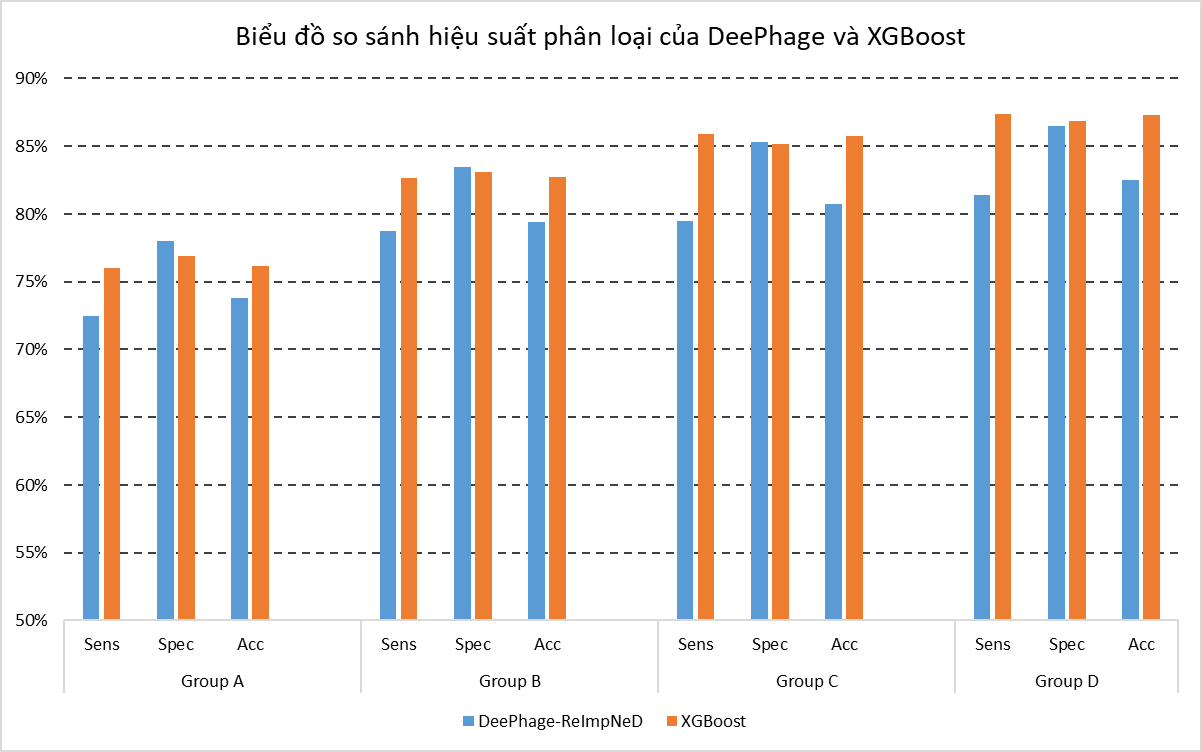
\includegraphics[width=1\linewidth]{figures/result_deephage_vs_xgboost.png}
    \caption{Kết quả hiệu suất phân loại của mô hình XGBoost trên tập dữ liệu xây dựng.}
    \label{fig:result_2}
\end{figure}

Hình \ref{fig:result_2} là biểu đồ so sánh hiệu suất phân loại của DeePhage và XGBoost trên tập dữ liệu mà nhóm báo cáo xây dựng. Có thể thấy, DeePhage cho kết quả tốt hơn 1 chút, khoảng từ 2\% - 5\% khi hơn XGBoost ở 2 chỉ số Sensitivity và Accuracy. Nghĩa là DeePhage cho khả năng nhận diện nhãn 1 và độ chính xác tổng thể cao hơn. Với chỉ số Specificity, XGBoost cho kết quả tốt hơn khoảng 5\%, nghĩa là khả năng nhận diễn nhãn 0 của XGBoost tốt hơn DeePhage.

